\documentclass[../Main.tex]{subfiles}

\begin{document}
\chapter{Finite Games/Nash Equilibria}
\textbf{Strategic form/normal form/matrix games:} Games in which all participants act simultaneously and without knowledge of other players' actions.
\begin{itemize}
    \item Set of players (agents)
    \item Set of actions 
    \item Set of payoff/utility functions
    \item Information structure players can access
\end{itemize}

\section{Finite Games}
\defn{Strategic form of game/Finite game}{A strategic forms game is a triplet $\langle \mathcal{I}, (S_i)_{i \in \mathcal{I}}, (u_i)_{i \in \mathcal{I}} \rangle$ such that
    \begin{itemize}
        \item[$\blacktriangleright$] $\mathcal{I}$: finite number of players, where $N = \mathcal{I} = \{1, 2, \ldots, n\}$
        \item[$\blacktriangleright$] $S_i$: set of actions (decisions, strategies) for player $i$
        \item[$\blacktriangleright$] $s_i \in S_i$: actions (decisions, strategies) for player $i$
        \item[$\blacktriangleright$] $u_i : S \longrightarrow \mathbb{R}$: the payoff (utility) function of player $i$, where $S = \prod_{i=1}^n S_i$ is the set of actions of all players
    \end{itemize}
}

\subsection*{Notation}
\begin{itemize}
    \item[$\blacktriangleright$] $s = (s_1, \ldots, s_n) \in S = \prod_{i=1}^n S_i = S_1 \times S_2 \times \cdots \times S_n$
    \item[$\blacktriangleright$] $s$: decision/action/strategy profile
    \item[$\blacktriangleright$] $s_{-i} = (s_1, s_2, \ldots, s_{i-1}, s_{i+1}, s_{i+2}, \ldots, s_n)$
\end{itemize}

\textbf{Strategy:} Complete description of how to play the game. Requires full contingent planning (full description how to play in every contingency).

\subsection*{General Setup of $n$-Player Finite Game}

\begin{itemize}
    \item[$\blacktriangleright$] Players: $n$-players with $i \in N = \{1, 2, \ldots, n\}$
    \item[$\blacktriangleright$] decision/action/strategy for Player $i$: $s_i \in S_i$
    \begin{itemize}
        \item[$\blacktriangleright$] $S_i$ is a finite set
    \end{itemize}
    \item[$\blacktriangleright$] $s = (s_1, \ldots, s_n) \in S = S_1 \times S_2 \times \cdots \times S_n$
    \begin{itemize}
        \item[$\blacktriangleright$] $s$: decision/action/strategy profile
    \end{itemize}
    \item[$\blacktriangleright$] $s_{-i} = (s_1, s_2, \ldots, s_{i-1}, s_{i+1}, s_{i+2}, \ldots, s_n)$
    \item[$\blacktriangleright$] Payoff function: $u_i(s_i, s_{-i})$ with $u_i : S \to \mathbb{R}$
    \begin{itemize}
        \item[$\blacktriangleright$] Each player has to maximize $u_i$ over $s_i \in S_i$
    \end{itemize}
\end{itemize}

\begin{itemize}
    \item[$\blacktriangleright$] Player 1 and Player 2
    \item[$\blacktriangleright$] $S_1 = \{1, \ldots, p\}$ finite set
    \item[$\blacktriangleright$] $S_2 = \{1, \ldots, m\}$ finite set
    \item[$\blacktriangleright$] $u_1: p \times m$ matrix
    \item[$\blacktriangleright$] $u_2: m \times p$ matrix
    \item[$\blacktriangleright$] Zero-sums game
    \begin{itemize}
        \item[$\blacktriangleright$] When $u := u_1 = -u_2$
        \item[$\blacktriangleright$] Player 2 plays minimizing $u$
    \end{itemize}
\end{itemize}

\begin{center}
    Player 2 \\
    \begin{tabular}{|c|c|c|c|}
        \cline{2-4}
        \multicolumn{1}{c|}{} & D & E & F \\
        \hline
        A & $(a, b)$ & $(c, d)$ & $(e, f)$ \\
        \cline{2-4}
        Player 1 \quad B & $(g, h)$ & $(i, j)$ & $(k, l)$ \\
        \cline{2-4}
        C & $(m, n)$ & $(o, p)$ & $(q, r)$ \\
        \hline
    \end{tabular}
\end{center}

\begin{itemize}
    \item[$\blacktriangleright$] Player 1 chooses row with respect to the first component
    $X_1 = \{A, B, C\}$
    \item[$\blacktriangleright$] Player 2 chooses column with respect to the second
    component $X_2 = \{D, E, F\}$
\end{itemize}

\section{Dominant Equilibrium: Optimality of Game}
For i player, a dominant strategy is one that yields the highest payoff, \textit{regardless of other players' actions}. A \textbf{Dominant Strategy Equilibrium} occurs when \textit{every} player has a clear best choice irrespective of others' and there is this no incentive for any player to deviate. (e.g., Prisoner's Dilemma). 

\textbf{Nash Equilibrium:} Set of strategies, for each player, such that \textit{no player can improve payoff by unilaterally changing only their own strategy} (assuming all players stick to chosen strategies). Note: a game can have multiple Nash equilibria and they don't always mean the best possible collective outcome for all players.

Every dominant strategy equilibrium is also Nash equilibrium. NOT the other way around though. 

\defn{Dominant strategy}{
A strategy $s_i \in S_i$ is dominant for Player $i \in N$ if
$$u_i(s_i, s_{-i}) \geq u_i(s_i', s_{-i}), \quad \forall (s_i', s_{-i}) \in S_i \times S_{-i}$$
where, $s_{-i}$ is collection of strategies chosen by all players except player i.
}

\defn{Dominant equilibrium}{
A strategy profile $s^* \in S$ is the dominant strategy equilibrium if for each Player $i \in N$, $s_i^* \in S_i$ is the dominant strategy.
\begin{itemize}
    \item[$\blacktriangleright$] We observe that "Confess" is the dominant equilibrium in Prisoner's dilemma game
    \item[$\blacktriangleright$] Rational players will choose the dominant strategy
\end{itemize}
}

\defn{Strictly dominated strategy}{
A strategy $s_i \in S_i$ is strictly dominated for player $i \in N$ if there exists some $s_i' \in S_i$ such that
$$u(s_i', s_{-i}) > u(s_i, s_{-i}), \quad \forall s_{-i} \in S_{-i}$$
\begin{itemize}
    \item[$\blacktriangleright$] Can obtain the dominant equilibrium by eliminating strictly dominated strategies (\textbf{iterated elimination of strictly dominated strategies (IESDS))}.
    \item[$\blacktriangleright$] Rational players do not choose the strictly dominated strategy
\end{itemize}
Therefore, if there exists another strategy $s_i'$ such that choosing $s_i'$  \textit{always} yields a strictly higher payoff for player $i$. regardless of what strategies other players $s_{-i}$ choose.}

\subsection*{IESDS} 

Method to simplify a game and find a solution/equilibrium. \\

Let $S_j^k$ be set of strategies for player j that have survived elimination up to iteration $k$. \\

Let $S_{-i}^k = X_{j \neq i}S_j^k$ be set of strategy profiles for players other than $i$ using strategies available at iteration $k$.\\

\textbf{Pseudocode:}
\begin{verbatim}
    Initialize S_i_current = S_i for all players i in N
Set strategies_eliminated_this_round = true

WHILE strategies_eliminated_this_round == true:
    Set strategies_eliminated_this_round = false
    FOR EACH player i in N:
        Let S_i_next_round = S_i_current
        FOR EACH strategy s_prime_i in S_i_current:
            Set is_dominated = false
            FOR EACH strategy s_double_prime_i in S_i_current (where s_double_prime_i != s_prime_i):
                Set s_double_prime_dominates_s_prime = true
                // Check if s_double_prime_i strictly dominates s_prime_i
                // against all combinations of opponents' current strategies S_minus_i_current
                FOR EACH strategy_profile_s_minus_i in S_minus_i_current: 
                    IF u_i(s_double_prime_i, s_minus_i) <= u_i(s_prime_i, s_minus_i):
                        s_double_prime_dominates_s_prime = false
                        BREAK // s_double_prime_i does not dominate s_prime_i w.r.t. this s_minus_i
                IF s_double_prime_dominates_s_prime == true:
                    is_dominated = true
                    BREAK // s_prime_i is dominated by s_double_prime_i
            IF is_dominated == true:
                Remove s_prime_i from S_i_next_round
                strategies_eliminated_this_round = true
        Set S_i_current = S_i_next_round // Update player i's strategy set for this iteration

Output: The final sets S_i_current for all players.
\end{verbatim}

\section{Nash Equilibrium: Optimality of Game}
\begin{itemize}
    \item[$\blacktriangleright$] N-player noncooperative game
    \item[$\blacktriangleright$] Rationality and optimality are key underlying assumptions
    \item[$\blacktriangleright$] No incentive to deviate once every player is in Nash
\end{itemize}
\defn{Nash Equilibrium (state)}{
The strategy profile $s^* = (s_1^*, \dots, s_n^*) \in S$ is called a Nash
equilibrium of the game if for all $i$, $i=1,2,\dots,n$,\[
u_i(s_i^*, s_{-i}^*) \ge u_i(s_i, s_{-i}^*), \quad \forall s_i \in S_i\]
Thus, no single player has an incentive to change only their own strategy. If player $i$ unilaterally deviates from $s^*$ to $s_i$, while $-i$ stick to $s^*$, player $i$ \textit{will NOT} achieve a strictly better payoff (either same or worse).
}
\defn{Best response function (tool)}{
The best response function \textbf{(correspondence)} $B_i(s_{-i})$ is defined by
$B_i: S_{-i} \to S_i$
$$B_i(s_{-i}) = \arg \max_{s_i \in S_i} u_i(s_i, s_{-i})$$
$$= \{s_i \in S_i \mid u_i(s_i, s_{-i}) \geq u_i(s_i', s_{-i}), \forall s_i' \in S_i\}$$
\begin{itemize}
    \item[$\blacktriangleright$]{It is sometimes correspondence, since given $s_{-i} \in S_{-i}$, there can be multiple $s_i \in S_i$}
    \item[$\blacktriangleright$] It is a multi-valued (set-valued) function
\end{itemize}
}

$B_i$ defines (set) strategy(s) such that player $i$'s payoff is maximized, \textit{given} $-i$ are playing $s_{-1}$.

Output of $B_i$ can be a set of strategies too if multiple yield same maximum payoff.\\

A strategy $s^* = (s^*_1,s^*_2,...,s^*_n)$ is \textbf{Nash Equilibrium} if every player's strategy in that profile is a best response to the strategies of all other players in that profile. Thus, $\forall i \in N$: $s^*_i \in B_i(s^*_{-1})$:

\propp{The strategy profile $s^* = (s_1^*, \ldots, s_n^*) \in S$ is a Nash equilibrium of the game if and only if $$s_i^* \in B_i(s_{-i}^*), \quad \forall i \in N = \{1, 2, \ldots, n\}$$}{
\begin{itemize}
    \item[$\blacktriangleright$] If part: since $s_i^* \in B_i(s_{-i}^*)$ for all $i \in N$, the result is true by definition
    \item[$\blacktriangleright$] Only if part: since $s^* \in S$ is a NE, the result follows from definition of the best response function
\end{itemize}
}

Current strategy maxed out payoff $=$ \textit{No} incentive to unilaterally change strategy.
\begin{center}
    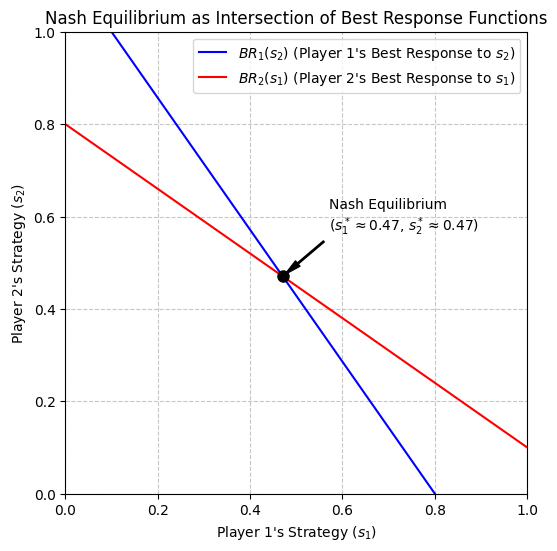
\includegraphics[width = 7cm, height = 7cm]{files/nash.png}
\end{center}

\defn{Nash equilibrium for two player game}{Simplified to two player game ($n=2$)

The strategy profile $s^* = (s_1^*, s_2^*) \in S_1 \times S_2$ is called a Nash equilibrium of the game if
\begin{align*}
    u_1(s_1^*, s_2^*) &\geq u_1(s_1, s_2^*), \quad \forall s_1 \in S_1 \\
    u_2(s_1^*, s_2^*) &\geq u_2(s_1^*, s_2), \quad \forall s_2 \in S_2
\end{align*}
}

Each player wants to choose their strategy to maximize their own payoff, keeping in mind that the other player is also trying to do the same.\\

\textbf{Core Idea: No Unilateral Incentive to Deviate (No Regrets)}\\

\textbf{e.g.,} Prisoner's Dilemma (PAyoff does not lead to best result at NE):\\

\textit{'The dilemma is that individual rationality (each prisoner choosing their dominant strategy to minimize their own sentence) leads to a collectively suboptimal outcome where both are worse off than if they had managed to cooperate. Even if they had agreed beforehand to Stay Silent, the incentive to betray the other for a chance at freedom (or a reduced sentence if the other also betrays) is very strong. This highlights the conflict between individual incentives and mutual benefit, and the difficulty of achieving cooperation in the absence of trust and binding agreements.'}

\section{Saddle-Point Equilibrium}

\defn{Saddle-Point Equilibrium}{NE for a \textbf{2-player zero-sum} game ($u = u_1 = -u_2$)

Strategy profile $s^* = (s^*_1, s^*_2) \in S_1 * S_2$ is a saddle-point equilibrium of 2-player game if
\begin{align*}
     u(s_1, s^*_2) \leq u(s^*_1, s^*_2) \leq u(s^*_1, s_2), \forall(u(s_1, s_2) \in S_1 * S_2
\end{align*}
\begin{itemize}
    \item[$\blacktriangleright$]{$u(s^*_1, s^*_2):$ \textbf{value of the game}}
\end{itemize}
}

\textbf{Minimax strategy (player 2 - minimizer of player's 1 payoff)}: For each column, player 2 identifies max. possible payoff Player 1 could achieve if player 2 chooses that column (assuming player 1 will try to maximize their payoff for that column). \textbf{Column Maximum***}

Player 2 then chooses strategy (column) that corresponds to the \textbf{minimum of these column maximums} = \textbf{Minimax value} of the game (From player 1's perspective, representing the maximum payoff player 2 is willing to concede. 
\begin{center}
    \textit{Maximin value (Player 1) = Minimax value (Player 2)}

    =

    \textit{\textbf{Value of the Game $(\mathbf{V})$}}
\end{center}

%%%%%%%%%%%%%%#############################################
%%%%%%%%%%%%%%#############################################
%%%%%%%%%%%%%%#############################################



\exm{Saddle Point in Pure Strategies}{

Consider the following \textit{PAYOFF MATRIX} for Player 1 in a 2-player 0-sum game.
Entries in matrix $=$ Payoff to Player 1. $(u= u1 =−u2)$

\vspace{1em} % Adds a small vertical space

% Payoff Matrix
\begin{center} % Center the table
\begin{tabular}{l | c c | c}
\toprule
                      & \textbf{Player 2:} & \textbf{Player 2:} & \\
                      & \textbf{Strategy Y1} & \textbf{Strategy Y2} & \textbf{Row Minimums} \\
\midrule
\textbf{Player 1: Strategy X1} & 4                     & \textbf{2}            & 2                \\
\textbf{Player 1: Strategy X2} & 3                     & 1                     & 1                \\
\midrule
\textbf{Column Maximums}      & 4                     & \textbf{2}            &                  \\
\bottomrule
\end{tabular}
\end{center}

\vspace{1em}

\textbf{Goal:} To find maximin and minimax values to identify saddle point:

\subsection*{1. Player 1's Maximin Strategy (Maximizing minimum guaranteed payoff)}
Player 1 looks at minimum payoff they could receive for each of their strategies:
\begin{itemize}
    \item If Player 1 plays Strategy X1, the minimum payoff is $\min(4, 2) = 2$.
    \item If Player 1 plays Strategy X2, the minimum payoff is $\min(3, 1) = 1$.
\end{itemize}
Player 1 wants to choose the strategy that maximizes this minimum payoff. The maximum of $\{2, 1\}$ is 2.
Thus, Player 1's maximin strategy is X1, and the \textbf{Maximin value = 2}.

\subsection*{2. Player 2's Minimax Strategy (Minimizing Player 1's maximum possible gain)}
Player 2 looks at the maximum payoff Player 1 could achieve for each of Player 2's strategies:
\begin{itemize}
    \item If Player 2 plays Strategy Y1, the maximum payoff Player 1 can get is $\max(4, 3) = 4$.
    \item If Player 2 plays Strategy Y2, the maximum payoff Player 1 can get is $\max(2, 1) = 2$.
\end{itemize}
Player 2 wants to choose the strategy that minimizes maximum payoff for Player 1. The minimum of $\{4, 2\}$ is 2.
Thus, Player 2's minimax strategy is Y2, and the \textbf{Minimax value = 2} (from Player 1's perspective).
}

\subsection*{Saddle Point and Value of the Game}
Since Maximin value (2) $=$ Minimax value (2) $\rightarrow$ Saddle point exists.\\

\textbf{$V$} $= 2$\\

Saddle point occurs at strategy profile where Player 1 plays \textbf{Strategy X1} and Player 2 plays \textbf{Strategy Y2}. The payoff at this point is \textbf{2} (to Player 1).\\

Looking at the entry `2` in the matrix (at the intersection of X1 and Y2):
\begin{itemize}
    \item It is the minimum value in its row (Row X1: values are $\{4, \mathbf{2}\}$).
    \item It is the maximum value in its column (Column Y2: values are $\{\mathbf{2}, 1\}$).
\end{itemize}
Dual property (minimum of its row and maximum of its column) is characteristic of a saddle point in a payoff matrix.

\subsection*{Stability of the Saddle Point (Connection to Nash Equilibrium)}{
At saddle point (X1, Y2):
\begin{itemize}
    \item If Player 1 (currently playing X1) unilaterally considers switching to Strategy X2 (while Player 2 continues to play Y2), Player 1's payoff would decrease from 2 to 1. Therefore, Player 1 has no incentive to switch.
    \item If Player 2 (currently playing Y2) unilaterally considers switching to Strategy Y1 (while Player 1 continues to play X1), Player 1's payoff would increase from 2 to 4 $=$ Player 2's payoff would change from -2 to -4 (zero-sum game), which is worse for Player 2. Therefore, Player 2 has no incentive to switch.
\end{itemize}
Since neither player has an incentive to unilaterally deviate from strategy profile (X1, Y2), saddle point is also a NE for the above 0-sum game.}\\

\textbf{Properties of Zero-Game:}
\begin{itemize}
    \item[$\blacktriangleright$] \textbf{Value is unique:}
    \begin{itemize}
        \item[$\blacktriangleright$] There is 1 value which is $=$ upper and lower values of the game.
    \end{itemize}
    \item[$\blacktriangleright$] \textbf{Order Interchangeability:}
    \begin{itemize}
        \item[$\blacktriangleright$] if $(x_1, x_2)$ and $(y_1, y_2)$ are saddle-point solutions, then $(x_1, y_2)$ and $(y_1, x_2)$ are also saddle-point solution
        \item[$\blacktriangleright$] $(x_1, x_2)$ and $(y_1, y_2)$ lead to \textit{same value} of the 0-sum game
    \end{itemize}
\end{itemize}

\section{Mixed Strategies and Mixed Nash Equilibrium}
\begin{itemize}
    \item[$\blacktriangleright$] Probability vector in strategy space
    \item[$\blacktriangleright$] Randomization of the strategy (action) space
    \item[$\blacktriangleright$] Payoff becomes expected value
\end{itemize}


%%%%%%%%%%%%%%#############################################

\end{document}

